\documentclass[12pt]{article}

\usepackage{amsmath}
\usepackage{amssymb}
\usepackage{graphicx}

\counterwithin*{equation}{section}
\counterwithin*{equation}{subsection}

\graphicspath{ {./images/} } 

\begin{document}
\section{Vectors and Surfaces}

\underline{Before}: \(y=f(x)\) \\%
\underline{After}: \(z=f(x,y)\) \\%
\(w = f(x,y,z)\) 


\underline{Quadric Surfaces}\\%
\underline{Ellipsoid}: $\frac{x^2}{a^2}+\frac{y^2}{b^2}+\frac{z^2}{c^2}=1$\\%
\underline{Elliptic Paraboloid}: $\frac{z}{c}=\frac{x^2}{a^2}+\frac{y^2}{b^2}$
\begin{itemize}
	\item Horizontal traces are ellipses
	\item Vertical traces are parabolas
\end{itemize}
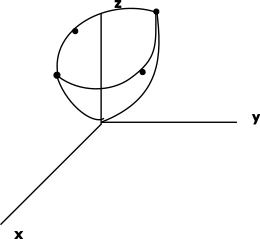
\includegraphics{parabaloid}\\%
\underline{Hyperbolic Paraboloid}: $\frac{z}{c}=\frac{x^2}{a^2}-\frac{y^2}{b^2}$
\begin{itemize}
	\item Horizontal traces are hyperbolas
	\item Vertical traces are parabolas
\end{itemize}
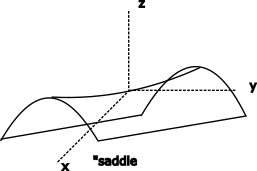
\includegraphics{saddle}\\%
\underline{Cone}: $\frac{z^2}{c^2}=\frac{x^2}{a^2}+\frac{y^2}{b^2}$\\%
\underline{Hyperboloid of One Sheet}: $\frac{x^2}{a^2}+\frac{y^2}{b^2}-\frac{z^2}{c^2}=1$\\%
\underline{Hyperboloid of Two Sheets}: $\frac{-x^2}{a^2}-\frac{y^2}{b^2}+\frac{z^2}{c^2}=1$\

\underline{Ex:} Put the equation in standard form and classify the surface.
\begin{align}
	\frac{x^2}{y^2}
\end{align}
	

\end{document}

